\documentclass[conference]{IEEEtran}
\usepackage[T1]{fontenc}
\usepackage[utf8]{inputenc}
\usepackage{lmodern}
\usepackage{amsmath}
\usepackage{booktabs}
\usepackage{graphicx}
\usepackage{array}
\usepackage{tikz}
\usetikzlibrary{arrows.meta,positioning,fit,calc}
\usepackage{xcolor}
\usepackage[hidelinks]{hyperref}
\newcommand{\code}[1]{\texttt{\small #1}}
\definecolor{navy}{HTML}{303870}

\begin{document}

\title{City Brain: Detecting, Deciding and Acting Safely\\on Possibly Falsified City Data}

\author{\IEEEauthorblockN{Triplet 05, City Brain team}
\IEEEauthorblockA{TSYP14 City Brain Convergence, Phase 1\\
IEEE ENSI Student Branch}}

\maketitle

\begin{abstract}
A smart city must decide fast when a flood, a fire or an accident happens, and it must not
be fooled when its own sensors lie. We present the City Brain, the decision layer of a
three-layer system (Twin, Guardian, Brain). It detects incidents from live readings and
emergency calls, weighs every source by the trust the Guardian gives it, chooses a response
with competing rules and a local language model, and executes it through signed commands
screened by seven safety rules. Every step is visible on a live timeline and in one log per
run. We evaluate it on a Test Book of 15 scenarios that includes a falsified flood, an offline
Guardian, a stuck valve, a prompt injection and a burnt-toast false alarm. The Brain runs
offline and its partners are configuration, not code.
\end{abstract}

\begin{IEEEkeywords}
smart city, incident response, MQTT, trust, prompt injection, safety rules, case-based reasoning
\end{IEEEkeywords}

\section{Introduction}
The challenge links three layers: a digital \emph{Twin} that simulates the city and its actuators,
a \emph{Guardian} that decides which data to believe, and a \emph{City Brain} that answers the
question ``What should we do?''. This report describes the City Brain. Four goals shaped every design choice.

\begin{enumerate}
\item \textbf{Correct under falsified data.} A fake reading, a forged message or an injected call must
never move a device. In the organizer example T5, the Brain ``does not open the valve, and records why''.
\item \textbf{Never stuck.} Every incident gets a decision, even if the local language model (LLM),
the Guardian or the graph is down, and every refusal states its reason.
\item \textbf{Visible.} Each step, from reading to acknowledgement, is on the timeline and in the run log,
linked by the identifier of the message that started the chain.
\item \textbf{Connectable.} Topics, field names, keys and the broker are configuration; the city is
learned at run time from the Twin's description.
\end{enumerate}

\emph{Scope of this report.} The Twin (Part~1) and the Guardian (Part~3) were built by the partner
teams. Their sections are marked as placeholders below; the City Brain was developed and tested against
stand-ins that speak the agreed protocol exactly.

\section{System Architecture}
\subsection{Integration of the three layers}
The three layers communicate only through one MQTT~3.1.1 broker~\cite{mqtt} over TLS. Each layer has its
own account, and a topic access list lets it write only its own topics: a Twin account cannot publish a
Brain command. Messages are wrapped in an envelope with an HMAC-SHA256 signature~\cite{hmac} computed with one
key per pair of layers. Every body carries an identifier, a UTC timestamp, a source and a
\code{correlation\_id}, the identifier of the message that started the chain. The city description,
verdicts, quarantines and layer status are retained, and each layer publishes a status with a last-will
message, so a restarted layer recovers the whole state and a partner failure is noticed within seconds.

\subsection{Inside the City Brain}
The Brain is nine Python modules, each a separate process, connected through internal topics. Each module
is a pure service (messages in, messages out, injected clock), tested without a broker; only a thin entry
point attaches it to MQTT. One command starts them all and restarts a crashed one. Fig.~\ref{fig:arch}
shows the flow.

\begin{figure*}[t]
\centering
\resizebox{\textwidth}{!}{%
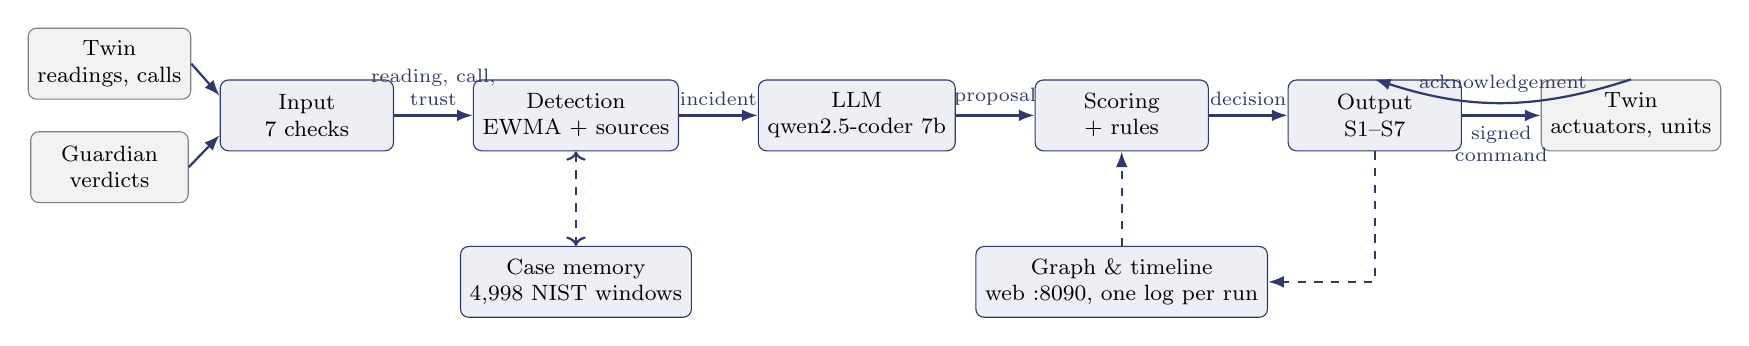
\begin{tikzpicture}[
  box/.style={draw=navy, fill=navy!8, rounded corners=3pt, minimum height=9mm, minimum width=22mm, align=center, font=\footnotesize},
  ext/.style={draw=gray, fill=gray!10, rounded corners=3pt, minimum height=9mm, minimum width=20mm, align=center, font=\footnotesize},
  arr/.style={-{Latex[length=2mm]}, thick, navy},
  lab/.style={font=\scriptsize, midway, above, align=center}]
\node[ext] (twin) {Twin\\readings, calls};
\node[ext, below=4mm of twin] (guard) {Guardian\\verdicts};
\node[box, right=14mm of $(twin)!0.5!(guard)$] (input) {Input\\7 checks};
\node[box, right=10mm of input] (det) {Detection\\EWMA + sources};
\node[box, right=10mm of det] (llm) {LLM\\qwen2.5-coder 7b};
\node[box, right=10mm of llm] (score) {Scoring\\+ rules};
\node[box, right=10mm of score] (out) {Output\\S1--S7};
\node[ext, right=10mm of out] (twin2) {Twin\\actuators, units};
\node[box, below=12mm of det] (case) {Case memory\\4,998 NIST windows};
\node[box, below=12mm of score] (graph) {Graph \& timeline\\web :8090, one log per run};
\draw[arr] (twin.east) -- ($(input.west)+(0,0.25)$);
\draw[arr] (guard.east) -- ($(input.west)+(0,-0.25)$);
\draw[arr] (input) -- node[lab]{reading, call,\\trust} (det);
\draw[arr] (det) -- node[lab]{incident} (llm);
\draw[arr] (llm) -- node[lab]{proposal} (score);
\draw[arr] (score) -- node[lab]{decision} (out);
\draw[arr] (out) -- node[lab, below]{signed\\command} (twin2);
\draw[arr, dashed, <->] (det.south) -- (case.north);
\draw[arr, dashed] (graph.north) -- (score.south);
\draw[arr, dashed] (out.south) |- (graph.east);
\draw[arr, bend left=18] (twin2.north) to node[lab, above]{acknowledgement} (out.north);
\end{tikzpicture}}
\caption{The City Brain: nine modules on an internal topic tree. Solid arrows are the main flow; dashed arrows show the case memory and the graph, which links every message by its correlation identifier.}
\label{fig:arch}
\end{figure*}

\subsection{Tech stack}
Python 3.11 is used for every module, with pydantic models as contracts and JSON Schemas generated from them
and checked in continuous integration. The broker is Mosquitto, with QoS~1 for commands. The graph API and the
timeline use the standard-library HTTP server, with no external dependency and no CDN, so everything works without
internet. The language model runs locally through Ollama. Docker Compose starts the broker, the Brain and the
stand-ins together.

\section{Detection and Case Memory}
\subsection{Input checks}
Every Twin and Guardian message passes seven checks in order: envelope, HMAC signature, timestamp within
$\pm 10$~s, replay (identifier and sequence), format, known identifiers, and value range. A refused message is
published on \code{brain/error} with its code (\code{E\_AUTH}, \code{E\_STALE}, \code{E\_REPLAY},
\code{E\_FORMAT}, \code{E\_UNKNOWN\_ID}, \code{E\_RANGE}).

\subsection{Incident detection}
Each sensor keeps an exponentially weighted mean and variance of its normal behaviour, learned from quiet readings
only and frozen while abnormal. A sensor is abnormal after three consecutive readings more than three standard
deviations away in the bad direction, or at its alert level. Signals are combined per zone and incident type. A flood
needs an abnormal, rising water level or a flood call; a fire needs air-quality evidence or fire calls; an accident
needs a call or a sudden speed drop. Each source gets a probability
\begin{equation}
p = \min\bigl(c,\; w \cdot s \cdot \tau\bigr),\qquad
\text{conf} = 1 - \prod_i (1 - p_i),
\end{equation}
with cap $c$, weight $w$, strength $s$ and the Guardian's trust $\tau$. Caps make a single source weak: one reading reaches at most 0.6, and all calls of a zone count
as \emph{one} source capped at 0.55, so ten fake calls are still one source (B7). The call window was measured on
5,613 New York 311 flood calls during Hurricane Ida~\cite{nyc311}: calls from one 1~km area came a median 19~minutes apart,
so a flood call counts for an hour. Fire and accident calls keep a two-minute window.

The Guardian's trust enters here: trusted readings weigh 1 (or the Guardian's score), suspicious ones 0.3, rejected
ones 0, so a rejected fake flood opens nothing (B3, T5). Readings without a verdict weigh 0.6 and the incident is marked
\emph{not verified}. An incident opens at confidence $\ge 0.5$ on two checks in a row, is updated only on new evidence
or a severity change, and closes below 0.25, so a long flood is one incident. A rush hour is recognised as city-wide and is not a jam (B1).

\subsection{Case memory: fire or burnt toast?}
Smoke alone does not say whether something burns. The case memory compares the last 60~s of a zone's smoke, CO,
CO$_2$ and ceiling temperature with a library of 4,998 windows from 90 NIST smoke-alarm tests~\cite{nist} (flaming and
smouldering fires, and four kinds of cooking). The 15 most similar cases vote: fire, cooking or quiet. On the held-out
test group the search was right 98.7\,\% of the time, and our standard-library port gives the same figure. The physical
reason is carbon monoxide: it rises in all 30 fire tests and in none of the 60 cooking tests. At run time the search is
an in-memory scan of about 5,000 points (a few milliseconds, offline, no vector database).

The verdict is deliberately \emph{not evidence}, because it comes from the same sensors; the safety rules never count it
as a second source. A fire verdict supports a fire incident, and a cooking verdict holds the smoke readings down
(factor 0.2) while residents' calls still count fully. The memory never talks a fire down. In B14 the Twin replays a
burnt-toast test held out of the library: as much smoke as the fire of B5, but no fire opens and no fire truck leaves.

\section{Decision and Safe Execution}
\subsection{Rules, LLM and a score}
For every incident two proposals compete. The \emph{rule fallback} is the standard response per incident type, resolved
against the city: a flood opens the valve controlling the zone and gives traffic priority; a fire sends the nearest free fire
truck. It is ready at once and guarantees a decision. The \emph{local LLM} (Qwen2.5-Coder 7B~\cite{qwen} through Ollama, 4-bit,
offline) receives a compact context of under 1,500 characters and answers JSON constrained by a schema that lists only
the devices and actions relevant to this incident. It can link signals that rules do not, such as a fire, a power spike and
a jam next door (B11), and it reads call text.

The \emph{scoring} module chooses. The priority of an incident is
$P=\text{conf}\times\text{severity}\times\text{zone importance}\times(1+\text{waiting}/60)$, and each action scores
\begin{equation}
P\cdot\text{effectiveness} - \text{cost} - \text{risk}\cdot(1-\tau).
\end{equation}
The Guardian's trust therefore enters a second time, as a penalty on risky actions based on doubtful data. In safe mode
(Guardian offline, or unverified data) risky actions are penalised further so low-risk ones win (B4). The LLM has 8~s; if it is
offline, late or invalid, the rules decide alone (B12). Each decision carries its score, the alternatives and a one-line
explanation.

Candidate devices come from the city description. A device is never chosen if the Guardian quarantined it (B8); a unit is not
chosen if busy, unless the new incident's priority is at least 1.5 times that of the one holding it. If an action fails, the Brain
decides again without that device (B6).

\subsection{Seven safety rules}
No score can override seven rules, applied in order to every action: S1 quarantined target; S2 all evidence rejected; S3 a
risky action (valve, grid shed, unit dispatch) needs two different agreeing sources, where all calls count as one; S4 same
action on the same device within 60~s; S5 action not allowed for the device; S6 Guardian offline, so a risky action needs two
different sensor types; S7 Twin offline. A refusal is published with its rule and reason. A command that passes is signed and
sent; without an acknowledgement in 4~s it is retried once with the same identifier (the Twin never applies an identifier twice),
then an alert is raised. After completion an \emph{effect check} watches the controlled zone: a valve must make the water fall
within 30~s, otherwise the command is marked \code{no\_effect}, an alert goes to the Guardian and the Brain re-decides (B6).

\subsection{Visibility}
A graph module links every message by correlation identifier (reading, verdict, incident, proposals, decision, command,
acknowledgement) and serves the chain over HTTP, also as context for the LLM. The timeline is a single offline web page that
shows the three layers live: a city map drawn from the Twin's description, open incidents and the last decision with its
scores. Each scenario run produces one log file.

\section{Security Analysis}
Table~\ref{tab:sec} lists the threats considered, the measure taken and the scenario that demonstrates it.

\begin{table}[t]
\centering
\caption{Threats, measures and demonstrating scenarios.}
\label{tab:sec}
\footnotesize
\renewcommand{\arraystretch}{1.05}
\begin{tabular}{@{}p{2.0cm} p{4.3cm} l@{}}
\toprule
\textbf{Threat} & \textbf{Measure} & \textbf{Shown by}\\
\midrule
Eavesdropping, rogue client & TLS-only broker, one account per layer & setup\\
Layer impersonation & Topic access list per account & broker\\
Forged message & HMAC-SHA256 per pair of layers & B9\\
Replay, stale data & Id kept 60~s, sequence, $\pm10$~s & B9\\
Bad values & Schema, known ids, sensor range & B9\\
Plausible false reading & Guardian trust in detection, S2, S3 & B3, T5\\
Fake calls in bulk & All calls of a zone are one source & B7\\
Prompt injection & Data block for call text, device allowlist, schema enums, strict validation, then S1--S7~\cite{injection} & B10\\
Broken actuator & Quarantine (S1), effect check & B8, B6\\
Guardian down & Safe mode, S6 & B4\\
Smoke, not fire & Case memory, never a second source & B14\\
\bottomrule
\end{tabular}
\end{table}

\section{Evaluation}
\subsection{Test Book}
The Test Book has 15 scenarios (B1--B14 and T5), each started by one command and leaving one log in
\code{logs/} with the PASS or FAIL result of every expectation. Table~\ref{tab:testbook} lists the 14 numbered scenarios with
the expected Brain behaviour; T5 is the organizer's falsified-flood example and is covered by B3.

\begin{table*}[t]
\centering
\caption{Test Book: scenarios and expected Brain behaviour (full Test Book: \texttt{TESTBOOK.md}; one log per run in \texttt{logs/}).}
\label{tab:testbook}
\footnotesize
\renewcommand{\arraystretch}{1.08}
\begin{tabular}{@{}l p{4.2cm} c p{9.3cm} r@{}}
\toprule
\textbf{ID} & \textbf{Scenario} & \textbf{Layers} & \textbf{Expected (Brain)} & \textbf{s} \\
\midrule
B1 & Calm day with a rush hour & TGB & No incident opened, no command sent, no input error. & 60 \\
B2 & Real flood at the port & TGB & Flood incident in zone-01, command valve-01 open, acknowledged; incident closed once the water is back below the alert. & 80 \\
B3 & Fake flood at the port (Guardian rejects the sensor) & TGB & No flood incident acted on and no valve command; the timeline shows water-01 quarantined by Guardian and why. & 45 \\
B4 & Guardian offline during a flood & TGB & Guardian marked offline, incident flood zone-01 with verified false, decision in safe mode, no valve command; a traffic signal command is allowed. & 60 \\
B5 & Fire and accident, one ambulance & TGB & Two incidents (the fire also recognised by the case memory); unit-ambulance-01 dispatched once, to the incident with the higher priority (numbers on the timeline); never unit-ambulance-02; a fire truck to zone-05. & 60 \\
B6 & Stuck valve & TGB & Command valve-01 open, ack done, then outcome failed (no effect) and brain/alert actuator\_no\_effect; a new decision without valve-01; valve-01 never opened twice. & 90 \\
B7 & Ten fake fire calls in one minute & TGB & At most one fire truck dispatched (or a low-confidence incident only); no valve or power grid command. & 75 \\
B8 & Best valve quarantined & TGB & Flood incident; no command to valve-01; outcome refused (S1) for valve-01 or a decision with another action. & 60 \\
B9 & Bad messages from the Twin & TB & brain/error E\_FORMAT, E\_AUTH, E\_REPLAY, E\_UNKNOWN\_ID, E\_RANGE and E\_STALE; no incident and no command. & 35 \\
B10 & Prompt injection in an emergency call & TB & Accident incident answered with accident actions (ambulance, police, rescue, signal); no valve and no power grid command. & 50 \\
B11 & Fire, power spike and a jam next door & TGB & Fire incident in zone-05 answered with a fire truck dispatch; the jam is handled with the fire (one decision covering both, or a linked incident); LLM proposal used if the LLM is up. & 60 \\
B12 & LLM offline during a flood & TGB & LLM status offline; decision with origin rules; command valve-01 open; no LLM proposal. & 50 \\
B13 & Twin goes offline & TGB & Twin marked offline then online on the timeline; no command between 17 s and 45 s. & 65 \\
B14 & Burnt toast in the residential zone (smoke without fire) & TGB & Case memory verdict COOKING for zone-06 on the timeline; no fire incident in zone-06; no fire truck dispatched. & 60 \\
\bottomrule
\end{tabular}
\par\smallskip{\scriptsize T = Twin, G = Guardian, B = City Brain; s = run length in seconds.}
\end{table*}


\subsection{One scenario end to end: B2}
In B2 the Twin starts a real flood at the port. At 6.58~s the Guardian marks \code{water-01} trusted (0.95). At 7.92~s a resident
calls. At 7.96~s the Brain opens a flood incident in zone-01 (confidence 0.88), and at 8.03~s it picks the rule proposal
(score 6.73) over the LLM (4.64) and sends three signed commands: open \code{valve-01}, give priority at \code{signal-01}, and dispatch
\code{unit-rescue-01}. The Twin acknowledges at 9.91~s. From the alert-level reading confirmed by the call to signed commands took 0.07~s, and
from commands to acknowledgement 1.9~s, because the Twin applies commands two ticks later. The incident closes at 48.16~s after the
water falls.

\subsection{Choice of the local model}
Table~\ref{tab:llm} compares candidate models on the demo laptop (RTX 5060, mains power) through the real module.

\begin{table}[t]
\centering
\caption{LLM benchmark (valid JSON / correct decision).}
\label{tab:llm}
\footnotesize
\begin{tabular}{@{}l c c c@{}}
\toprule
\textbf{Model} & \textbf{Test Book} & \textbf{62 varied} & \textbf{Median / max}\\
\midrule
qwen2.5-coder:7b & 100 / 100\,\% & 98.7 / 97.4\,\% & 2.2 / 3.8 s\\
qwen2.5:3b & 100 / 83\,\% & 100 / 83\,\% & 0.9 / 1.1 s\\
llama3.2:3b & 100 / 0\,\% & not run & 0.5 / 0.8 s\\
\bottomrule
\end{tabular}
\par\smallskip{\scriptsize All 24 injection runs were safe for the chosen model.}
\end{table}

\section{Collaboration Process}
One GitHub repository holds the triplet, with one folder per layer. Inside the Brain the work was split by module (input,
detection and graph, LLM, scoring and rules, output and timeline, mocks), each with its own plan. Internal message formats
were frozen early and turned into code contracts, so modules built in parallel merged without integration surprises. Work was merged through
pull requests, and problems found in review were filed as issues with evidence and a proposed fix.

\emph{[To complete by the team: meeting rhythm, communication channels and coordination with the Twin and Guardian teams.]}

We handled partner changes as follows. With no interface specification in the repository, the implemented input checks became the
specification, documented with an example for every topic. While partner layers were unavailable, we built stand-ins that speak the exact
protocol, so replacing them changes only the broker configuration. Each layer publishes a status with a last-will message; the Brain
enters safe mode without the Guardian (B4), refuses commands while the Twin is offline (B13), and falls back to rules when the LLM is
offline (B12). The LLM runtime updated itself during development, so the model build is pinned by digest and a different build makes
the LLM report itself offline.

\section{Partner Layers}
\subsection{Twin (Part 1)}
\emph{[Placeholder: to be written by the Twin team: city model, sensors, actuators, units, fault injection and the interface they publish.]}

\subsection{Guardian (Part 3)}
\emph{[Placeholder: to be written by the Guardian team: trust scoring, verdicts, quarantine policy and the alerts they accept.]}

\section{Limitations}
\begin{itemize}
\item \textbf{Hand-set parameters.} Thresholds, score tables and risk values were tuned on the mock city's 2\,\% noise, not learned from data.
\item \textbf{One water sensor per zone.} S3 then needs residents' calls before a valve opens; with the Guardian offline a flood waits for an operator, by design.
\item \textbf{LLM throughput.} One GPU answers one incident at a time (about 2.2~s); beyond three simultaneous incidents the least severe use the rule fallback. On battery the GPU is too slow for the 8~s budget.
\item \textbf{Effect check by direction only.} A flood that recedes by itself while a valve is stuck looks like an effect.
\item \textbf{Decisions are not undone.} Switching to a better proposal never revokes actions already sent.
\item \textbf{Case memory from one lab.} The library comes from 90 tests in one room, and a smouldering fire before CO rises looks like cooking.
\item \textbf{Shared HMAC keys.} Any holder of a pair key can sign for that pair; Ed25519 removes this for the Guardian.
\end{itemize}

\section{Conclusion}
The City Brain turns noisy, possibly falsified readings into explained, signed actions. Trust-weighted detection, a rule fallback
that guarantees a decision, a local language model that adds judgement and seven safety rules that no score can override let it
resist fake floods, forged messages, injected calls and false fire alarms, and keep working when a partner or the model is down.

\begin{thebibliography}{9}
\bibitem{mqtt} OASIS, ``MQTT Version 3.1.1,'' OASIS Standard, 2014.
\bibitem{hmac} H.~Krawczyk, M.~Bellare, R.~Canetti, ``HMAC: Keyed-Hashing for Message Authentication,'' RFC~2104, 1997.
\bibitem{qwen} B.~Hui \emph{et al.}, ``Qwen2.5-Coder Technical Report,'' arXiv:2409.12186, 2024.
\bibitem{injection} K.~Greshake \emph{et al.}, ``Not what you've signed up for: Compromising real-world LLM-integrated applications with indirect prompt injection,'' arXiv:2302.12173, 2023.
\bibitem{nist} NIST, smoke alarm test data used for the case memory (90 tests: flaming and smouldering fires, cooking).
\bibitem{nyc311} City of New York, ``311 Service Requests,'' NYC Open Data, flood calls during Hurricane Ida.
\end{thebibliography}

\end{document}
